\documentclass[a4paper]{llncs}

\usepackage{times,verbatim} % Please do not comment this

\usepackage[]{graphicx}
\usepackage{url}

\begin{document}

\pagestyle{empty}

\mainmatter

\title{Experiments of Discovery Services Interconnection~\protect\footnote{This work is
  carried out within the framework of a french national project: ANR
  WINGS.}~\protect\footnote{This work is supported in part by the french CPER Basse-Normandie.}}

\titlerunning{Experiments of Discovery Services Interconnection}

\author{Adrien Laurence\inst{1}, J\'{e}r\^{o}me Le Moulec\inst{1} \and Jacques Madelaine\inst{1} \and Ivan Bedini\inst{2}}

\authorrunning{Adrien Laurence et al.}

\institute{GREYC -- CNRS UMR 6072,\\
Bd Mar\'{e}chal Juin,
F-14000 Caen, France\\
\email{\{jerome.le\_moulec, jacques.madelaine\}@info.unicaen.fr}
\and
Orange Labs.\\
42, rue des Coutures,\\
F-14000 Caen, France\\
\email{ivan.bedini@orange-ftgroup.fr}}

\maketitle

\begin{abstract}

This paper presents a platform called IOTA, an open implementation of the
EPCglobal architecture. It aims to collect and to store events about object involving
in a given supply chain.  Iota uses a Petri net simulator to emulate the lower
layers including the RFID readers.  Iota focuses on the design of a non
centralized Discovery Services and experiments in a real network environment.
This paper presents the experiments of a solution for distributed Discovery
Services and its impact on the overall architecture in terms of performance issues.

\end{abstract}

\section{Introduction}

The usage of RFID tags is now so common that we urgently need for efficient
lookup services among the events tracing the tags. We currently develop a
platform called IOTA (Internet Of things Application) in order to experiment
events storage and lookup services. It is deployed over four locations linked
with a real wide area network. 

IOTA satisfies the EPCglobal requirements and implements the already published standards.
If the storage and the data sharing of the events capture is standardized, the
data search and the lookup services are still at a proposal level. At the
moment, these propositions does not take distributed control into account. This
option raises some political difficulties as organizations generally wish to
keep control over these data.
We propose a solution to avoid monolithic discovery services. This solution
has a overhead cost in terms of  additional messages and storage that we study
in this paper. 
This paper presents the results of the first tests we have run on the IOTA platform.  

The paper is organized as follows. Section 2 presents the Epcglobal
architecture organized in layers. Section 3 recalls the different strategies
for decentralized discovery services. The use case used for our simulation is
described in Section 4. Section 5 presents the architecture of our platform and
details the non standard components we have created. Section 6 discusses the
tests results. Finally, we give in Section 7 some open issues.
   
\section{EPCglobal Architecture Overview}
\label{sec:epcglobalarch}


The EPCglobal architecture is composed of dedicated components grouped in four
layers (see Figure \ref{fig:epcgloblalayers}). The lower layer deals with RFID
tag reading. Each tag contains a unique Electronic Product Code (EPC). The ALE
of the lower layer is in charge of editing the so called EPC \emph{events}. The
main goal of the upper layers will be to store and manage efficiently these
events.

\begin{figure}[htbp]
  \centering
  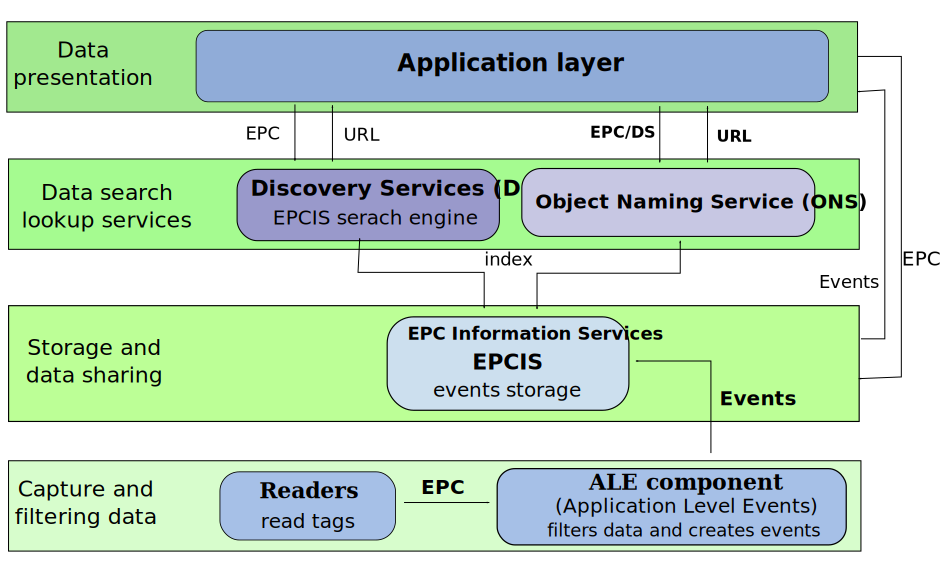
\includegraphics[width=0.8\textwidth]{iota_visuel/epcglobal_archi.png}
  \caption{EPCglobal layers}
  \label{fig:epcgloblalayers}
\end{figure}

As soon an event is created, it is first send to the local Electronic Product
Code Information Services (EPCIS). That component uses a persistent database to
store the events and offers a fully standardized query interface to the upper
layers~\cite{epcis}.
It also manages master data containing necessary context
for interpreting the event data.

The next layer is in charge of indexing the EPCIS in order for an application
to locate the EPCIS that stores events about a given EPC code. The first component of this
``Data Search Lookup Services''  is the Object Naming Service (ONS).
It aims to provide addresses for product
classes. Actually, ONS does not deal with EPC code but solely  with object
class numbers.  For example if company A manufactures a product with the EPC
code: \url{urn:epc:id:sgtin:a.b.x}. The ONS system will provide the EPCIS
address of the product manufacturer (company A) for the class:
\url{urn:epc:id:sgtin:a.b}. It will also provide other information like a web
site address.
In order to locate all the potential sources of information for a given EPC
the Discovery Services (DS) indexes the EPCIS. Unlike web search engines that
crawl the web to gather information, the DS receives information directly by
the EPCIS layer that submits information about an event related to a given
code. This design is preferred for evident access control issues. 

Last the application layer may implement commercial services such as carbon footprint
computation or counterfeit tracking. 

If the components of the two lower layers are fully standardized, only the ONS
is now standardized in the upper layers. The ONS architecture mimics the
Internet DNS architecture. It is organized as a strict hierarchy. The benefit
is that we can use to implement the ONS, the same software as for the DNS,
namely BIND.%~\cite{bind}.
Unfortunately, the ONS, as the DNS, is based on a single root. If this is
acceptable for the DNS, as we don't create everyday an Internet top level
domain, this is absolutely not the case for the ONS. Some proposals exists for
a Multi Root ONS~\cite{DBLP:conf/iot/EvdokimovFG08,wings}.

The other component responsible of the lookup services is the DS. 
For a given EPC code it can deliver all EPCIS addresses dealing with that
code. EPCIS enforces access control policies. But even if the EPCIS denies the
access to the event, the fact that a given EPCIS holds a code may be a
disclosure of private information. Therefore, DS implementations must also
achieve access control policies.  

\section{Strategies for Multi DS}
\label{sec:strategies}

As mentioned above, a realistic EPC network should have multiple DS
components. However the DS Standard is still in development by the EPCglobal
Data Discovery Joint Requirements Group and the architecture and
interconnection of distributed DS is an open question. In the paper
\cite{AI-LEMOULEC-2009}, we described three alternative solutions to the
problem of several Discovery Services interconnection in order to offer a
distributed lookup architecture.

The first alternative was called ``DS like a Peer''. It explained how to
reference the events stored in several EPCIS servers using a distributed
hash table. Each EPCIS that contains information on a particular EPC publishes
it on the Peer2Peer cloud. A client can then query the P2P network thanks to one
front end DS server and retrieves all the EPCIS addresses. The main drawback of
this solution concerns the security and access control policy aspects and the
capability for the P2P network to prevent efficiently from competitive intelligence.

The second solution, called ``DS like a router'' is based on the dynamic
linking of the EPCISs. The ONS component in the EPCglobal architecture provides
the address of the first EPCIS of the chain for a given EPC. If each EPCIS is
linked for this same given code, it is possible to retrieve the information by
querying each chained EPCIS one after the other. The main problem is to create
the links between the different EPCIS. In fact, a particular product may take a
different route and could be lost unless the chaining process is dynamic.  To
realize this, we proposed to use an XML rooting network. After analysis, it
appears that this solution is much to sensitive to server failure.

The last proposal called ``DS indexing DS'' looks simpler and more efficient to
realize the distributed indexing mechanism. The main aspect of this
implementation is the introduction of a new concept, the \emph{referent DS}. Indeed,
for each product class (i.e. EPC without serial number) a NAPTR entry is
defined in the ONS system with the code and  the address of a particular DS server. This
server, that we call the \emph{referent} will not only index the EPCIS like
every DS but will also index other DS servers for all the events using a code
belonging to this EPC class. 

During the indexing process, each DS that receives information about a
particular EPC, queries the ONS system in order to retrieve the referent DS
address.  Two different cases takes place whether the DS is the referent DS for
this code or not. The DS can easily notice he is the referent in comparing its
own address with the address it received from the ONS. If it is the referent
DS, it just indexes normally the EPCIS.  Otherwise, on top of indexing the
EPCIS, it publishes a new DS entry to the referent DS using the same process as
if it was an EPCIS (on the same interface and with the same protocol).

As a result, during the lookup process, the client queries the ONS system for a
particular EPC class, in order to
retrieve the referent DS address  and queries it in turn.
The response may contain according to the standard several EPCIS, and/or
according to our proposal, several DS addresses. The client can then
query again these new discovered DS to retrieve other EPCIS addresses
containing information events about that code. When
there is no more DS address to be queried, the client has collected all the
information sources that he needs to track the given object.

In this paper we give the result of the experiments conducted on our platform
that implements this third proposal (DS indexing DS).  

\section{The Use Case}

The use case we consider to validate our multi DS strategy with a referent DS
is a simplified assembly-line production of jeans. All the usual supply chain
partners are modelled: three raw material producers, two manufactures, three
wholesalers and a retailer. Each partner has his own EPCIS that publishes its
events to a Discovery Service. 

This use case is not totally realistic. By example, we have only one retailer. In fact, we
designed it especially to stress and augment the need of communication between
the components  in order to validate our multi DS schema. This section describes the
events generated in this use case by each partner.

\subsection{Raw Material Producers}

In the use case, we suppose that a pair of jeans is composed of denim fabric
(produced by producer 1), buttons (produced by producer 2) and zips (produced
by producer 3)~\footnote{Not mentioning sewing thread and rivets.}. If all the
three producers EPCIS are located on the GREYC servers, their referent DS is
located respectively at the GREYC for producer 1, at the CERTIC for producer 2
and at ORANGE labs for producer 3 as depicted on Figure \ref{fig:iota}.


Once made, each raw material is equipped with a new RFID tag containing a
unique EPC code. It is detected by a first reader while it enters the
producer's warehouse.  The reader publishes an event to the EPCIS with the
action ``ADD''. To indicate it is the first time the EPC is detected on the
supply chain, the event business step is ``encoding''.  The second reader
detects the good when it is loaded on a truck for delivery.  The event
published has the value ``OBSERVE'' for action and the business step
``departing''.


\begin{figure}[htb]
\centering
\includegraphics[width=0.7\textwidth]{iota_visuel/iota_log_paper.png}
\caption{IOTA deployment}
\label{fig:iota}
\end{figure}
%\begin{figure}[htb]
%\centering
%\includegraphics[width=0.8\textwidth]{iota_visuel/iota_network.png}
%\caption{IOTA deployment}
%\label{iota}
%\end{figure}

\subsection{Manufactures}

The manufacture is supposed to receive the raw material and to assemble the final
product: the jeans. For this step, there are two manufactures whose EPCISs are
located in the CERTIC, but DS for manufacture 1 is located at the GREYC.
 
Each manufacture has three readers. The first one tracks the arrival of raw
materials. It generates an event with action ``OBSERVE'' and business step
``arriving''.  As soon as the jeans are made, a new RFID tag with a new EPC is
created by the manufacture RFID printer and allocated to the jeans. When the
jeans get through the reader, it doesn't publish a simple event to the
EPCIS. Indeed, in order to trace the materials origins, the reader has to send
an \emph{aggregation} event encapsulating not only the jeans EPC code, but also
the EPC codes of the raw materials used for its making.

Finally, a third reader tracks goods when they leave the manufacture to go to
the wholesaler. The event has the action``OBSERVE'' and the business step
``departing''.


\subsection{Wholesalers}

The wholesaler has two readers, one located at the delivery arrival and the
other one at the delivery departure. 
Three wholesalers are present in this use case, the wholesaler 1 is
located in the CERTIC and the wholesaler 2 and 3 are located in Orange
Labs. Each one uses a DS located on a distant site. 

\subsection{Retailers}

The retailer is the final peer of the supply chain, thereby his part is to
receive goods from the wholesalers and to sell them to the end
customers. The retailer has two readers like wholesalers. 

If the first reader tracks goods arrival as for manufacturers, the second one
is rather special.  It is the last reader of the supply chain.  We suppose that
the tag is deactivated at this step when the jeans is sold out.  Therefore, the
event triggered by this last reader contains the action ``DELETE'' with the
business step ``sold''.  The action ``DELETE'' means that no more event
concerning this EPC code will be sent in the EPC network.

%As we can see in Figure \ref{fig:iota}, there is one retailer located in a dedicated server in Orange
%Labs and it publishes his events to the Orange's DS.

To finalize the description of the use case, we must just state that the
referent DS for raw material is Ds-Unicaen and the one for jeans is
DS-Certic. These two facts will be used to compute the number of
messages exchanged during the tests analyzed in  Section \ref{sec:tests}.

\section{IOTA Architecture}

IOTA is a platform of an EPCglobal
network that realizes the whole scenario depicted above. Each peer of this
network belongs to a layer of the EPCglobal architecture as presented on the
Figure \ref{fig:epcgloblalayers}. In this section, we describe the peers
actually installed in IOTA and the communication between them.

IOTA is a platform gathering nine EPCIS, three DS and the ONS system
distributed over three locations (the GREYC laboratory and the CERTIC from the
university of Caen Basse-Norman\-die and Orange Labs Caen). Figure
\ref{fig:iota} shows the deployment of these components by the different
partners. This platform puts the EPCglobal components in a realistic situation
according to the network heterogeneity and problems (firewalls, links
speed\ldots{}). Only the EPCglobal upper layers are deployed in IOTA. The
components located in the capture layer (readers and ALE) are simulated using a
Petri net application described section~\ref{sec:simulator}.

\subsection{General Architecture}

Figure \ref{archi} depicts the IOTA architecture modules with respect to
the EPCglobal framework. Moreover the picture shows the components and their
connections that we have developed in order to realize and validate our multi
DS implementation. If it uses, as explained in this section, standard component
implementation for EPCIS and ONS, it uses an implementation of ESDS-1.0
specifications for the DS and an original component: the IS2DS gateway. The
lower layer is emulated with the PetriNet simulator. Last we use a special
application layer component in order to validate and test the whole
implementation; the validator.


\subsection{Electronic Product Code Information System (EPCIS)}
\label{subsec:EPCIS}

Several EPCIS implementations are currently available, like Fosstrak~\cite{fosstrak},
Seres~\cite{seres}, BizTalk~\cite{bizTalk}, Bent System~\cite{bent} or IBM~\cite{IBM}. In our
implementation we use Fosstrak that is an open source RFID software platform
that implements the EPC Network specifications. The Fosstrak application used
in IOTA contains the EPCIS repository. It offers two interfaces: one for capture and the other for
query. The Fosstrak EPCIS capture interface uses a simple REST protocol, whereas the
query interface is a full SOAP implementation of the EPCglobal EPCIS
interface standards~\cite{epcis}. Among the several query types it allows, there is subscription.
Subscription allows a client to request one EPCIS repository in order to
retrieve periodically the last inserted filtered events. We use this facility
to connect a DS server to an EPCIS.

In order to insure the independence from EPCIS and DS standards, we developed a
new middleware component, called \emph{IS2DS Gateway}, that realizes this
interconnection. 
It implements the EPCIS query client and subscribes to one EPCIS following a
given refresh rate. As it is, in IOTA, each IS2DS application receives minutes by
minutes the new inserted events from the EPCIS it subscribed to. This event
list can be filtered by the EPCIS owner given new parameters to the
subscription such as business step, read points\ldots{} IS2DS has its own
private database used to store in these events until they are published to the
DS server. This prevents the component to be sensitive to server failures.

\begin{figure}[htb]
\centering
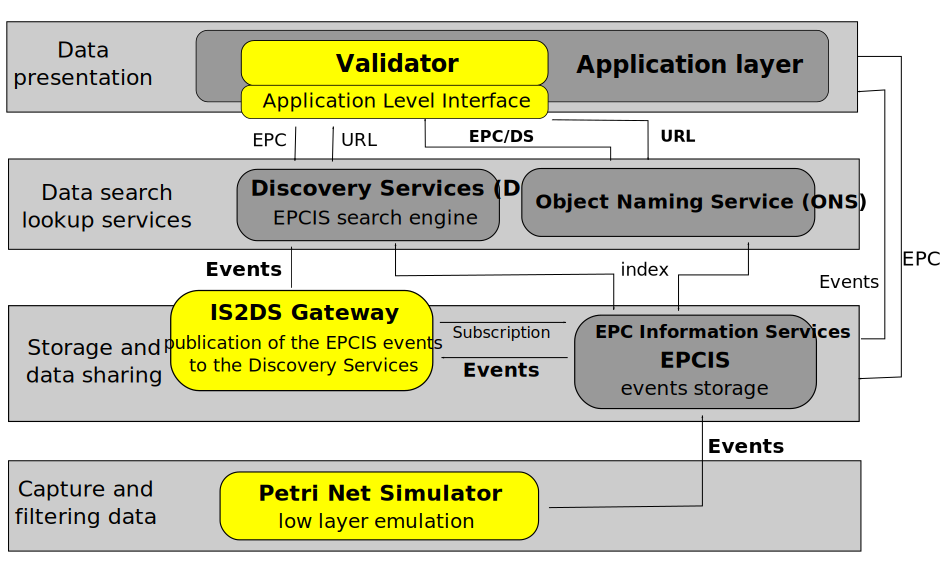
\includegraphics[width=0.7\textwidth]{iota_visuel/iota_archi_funct_grise.png}

\caption{IOTA functional architecture}
\label{archi}
\end{figure}

We count nine EPCIS installed in the IOTA platform. Each EPCIS has its own
IS2DS gateway connected to several DS servers. Figure \ref{fig:iota} shows the
deployment over the three organizations. Three EPCISs (with their gateways) are
installed in the GREYC laboratory, three others in the Certic and the last
three are installed in Orange Labs Caen.

\subsection{Discovery Service (DS)}
\label{subsec:DS}

The Discovery Services component is not currently standardized by
EPCglobal. The instance we use in IOTA have been developed by Orange and the
GREYC laboratory partners. The core component (DS repository) is based on the
EPCglobal requirements. The capture and query
interface is a SOAP 
implementation of the ESDS-1.0 protocol proposed by Afilias~\cite{afilias}. 
%% non distribu\'e
The IS2DS application that we have just presented, uses this same protocol to
publish its events to the DS. It starts by identifying itself using the EPCIS
account created in the DS. It then, publishes its events using the \texttt{eventCreate}
method. In order to improve the performances, we have extend the ESDS protocol
by allowing a single SOAP message to contain several published events. As
described in Section~\ref{sec:strategies}, the referent DS must also index the
other DS servers indexing events concerned by the EPC codes it is referent
of. The data exchange protocol used in that case is still the same ESDS-1.0
as for the EPCIS publications. The only difference is that DS uses a DS account
instead of an EPCIS account.

The access control policy module is part of the DS core component. Each EPCIS
connected to a particular DS must, as a first step, create an account. In this
account, the partner can create supply chains (SC) and associate other
partners. For example, partner A creates a new SC ``SC1'' and associates
partner B. Then partner B will be allowed to retrieve all the indexed
information inserted by partner A. Partner A can also add some filters. For
example, he can add a BizStep filter to ``SC1'' in order to share only the
events with the given business step value.  We have currently four allowed
filters on: business step, event class, epc and event time period.  

We count three DS servers in IOTA. Each site (GREYC, CERTIC and Orange Labs) has its own instance.

\subsection{Object Name Service (ONS)}
\label{subsec:ONS}

The ONS architecture is based on the DNS one. The software used in IOTA to
realize the operation is Bind. Currently, we have only one local ONS instance
connected to the GS1 ONS root. The IOTA project is part of the WINGS project
gathering the partners Orange labs, GS1 France, Afnic, the LIP6 and the GREYC
laboratory. This project aims to develop a distributed ONS architecture to
prevent from a centralized one like in the DNS architecture. In this context,
the IOTA platform will host in the next few months one root ONS and an other
local one.

The IOTA local ONS is currently hosted by Orange Labs on a dedicated server.

%Next section presents the lower layer IOTA component.



%In Figure \ref{archi}, we can see three components (the PetriNet Simulator, the Validator and the
%IS2DS gateway) that we haven't yet mentioned. The PetriNet Simulator and the Validator will be
%explained in the next sections. However, the IS2DS gateway is a choice of the middleware
%architecture we have done. In fact, this component aims to publish the EPCIS events to the Discovery
%Services and to respect the EPCglobal specifications. To this end, the IS2DS gateway
%subscribes to the EPCIS to retrieved all the shared events in a first time and in a
%second time publishes them to the DS. We have used the subscriptions system that is present in the
%EPCglobal specifications to resolve the events publication between the EPCIS and the DS.
%
\subsection{The PetriNet Simulator}
\label{sec:simulator}

Only the upper layers of the EPCglobal specifications are implemented in
IOTA. There is neither physical readers nor real ALE components. In fact, this
allows to easily create as many scenarios as we want. It is useful to create an
application that is able to simulate a lot of readers, ALE components and to
publish a lot of events to as many as EPCIS that we dream of.

In order to realize a scenario, we have developed a IOTA supply chain
simulator. It is based on a Petri net~\cite{Kindler99thepetri} where the places,
transitions and tokens model respectively warehouses, readers and objects
identified by a unique EPC. The transition fire emulates an ALE component,
setting additional information to the event such as read point, business step,
disposition, action, timestamp, GPS localization.  Then, the event is sent to
the EPCIS address specified in the transition configuration.

Some extensions have been developed in order to add constraints to the
simulated supply chain. For an ``arc'', we can defined a specific number of
tokens needed to activate the next transition. It's used for example to
simulate the departure of a truck containing several objects.  Extensions for
places have been also defined. The user may specify how many products can be
stored in a given place. The ``EPC Generator'' option specifies that this place
generates tokens with new unique EPCs. When this option is
activated, the user can specify the number of tokens and the EPC class of the
generated EPCs.

In order to realize  validation tests on the IOTA platform, we need to prove
that all the generated events have been stored in the right EPCIS servers. During
the object transportation process, all the information concerning their
evolution is stored by the simulator.  The user can specialize a place as
``Event File Saver''.  When a token arrives in that particular place, its
progression is stored in a log file.  The user can also specify if a place is
used as ``EPC Deactivator''.  It simulates the fact that the product has been
sold to the final consumer and the tag has been consequently deactivated. This
last possibility solves a technical limitation. Indeed when the user wants to
simulate a very large supply chain with a lot of object and readers, for a long
time, the application must keep the travel of all the objects in its
memory. The memory grows up continuously and the simulator may fall down
because of a memory leak. To prevent this situation, it is advisable to switch on
this option at each end point of the simulated supply chain.

The goal of such a simulator is also to perform measures of the servers
response times during the events capture process.  Whenever an event is sent,
the EPCIS server response time is recorded by the simulator. It uses one
different file by server.  

\subsection{The Validator}
\label{subsec:validator}

All the generated log files of the simulator may be further used by the
IOTA Validator. It is a Java application that queries the platform in order to
retrieve the events stored in the different servers and to validate their right
emplacement.  In order to achieve this task, the validator takes as input the
network topology, i.e. the addresses of the EPCISs, DSs and ONSs as well as
their inter-connections. It then uses the standard application interface
described in Section~\ref{subsec:EPCIS} and~\ref{subsec:DS} to retrieve all the
events in the different DSs and EPCISs.  
Afterwards, it has only to compare the list of the collected events
to the list stored in the simulator. Finally, a report is built for each generated
objects.

The report may also incorporate in the report the response times needed by the
simulator and stored in the log files. 
Unfortunately, as the simulator does not use directly the DS, it is unable to monitor
precisely the response time of the DS messages needed for the indexing process.
% \emph{*** tbc***}


\section{Tests Results}
\label{sec:tests}

In order to validate and test our architecture, we run several tests of events
generation with the simulator. In this section, we first count the expected number of events
generated and the number of messages exchanged between the components.
We then present the number of events and the EPCISs response times
measured by the simulator. 

\subsection{Formal Analysis of the Use Case}

We count, in this section, the number of messages needed by the events recording and
indexing processes. 
 
Each time a RFID tag is detected by a reader, one event is sent to the
EPCIS. The EPCIS will publish it to the DS using the IS2DS gateway leading to
two messages: one from the EPCIS to the IS2DS and one from the IS2DS to the
DS. In case the DS is not the referent DS for this code, a message concerning
this event is forwarded to the referent DS. These rules lead to the figures
presented in table \ref{tab:nbEvents} for the three producers.
 
For the manufacturers, the situation is not so simple. They receive raw
materials grouped ten by ten in a truck. Thus, only one event, referencing ten
EPC codes, is generated when a reader detects ten objects. This is the case for
the three different types of raw material. After a jeans is assembled, a new
tag is produced. This is recorded through an aggregation event issued by the
second reader. A last event is send to the EPCIS when the jeans leaves the
factory. This makes 2.3 events for a pair of jeans.  These events  are all forwarded to
the DS but a DS event must concern only a single EPC code in the ESDS-1.0
protocol. This lead, for a final product, one event per raw material item, plus
four events because the aggregation event concerning four different EPC codes
must be split, plus the final one. This makes a total of $3 + 4 \times 1 + 1 = 8 $ messages
from the IS2DS to the DS. The number of DS to DS messages depends on who is the
referent DS for the class code as for the producers.

\begin{table}
\caption{Number of events generated by each peer.}
\begin{center}
\begin{tabular}{|l|c|c|c|c|c|}
 \hline
 \multicolumn{1}{|c|}{Peer} & Number of & \multicolumn{3}{c|}{Number of events}  & Probability \\
 \cline{3-5}
          & Readers & EPCIS/IS2DS & IS2DS/DS & DS/DS  & being used\\
 \hline\hline
 Producer 1 & 2 & 2 & 2 & 0  & 1 \\
 Producer 2 & 2 & 2 & 2 & 2 & 1 \\
 Producer 3 & 2 & 2 & 2 & 2 & 1 \\
 \hline
 Manufacturer 1 & 3 & 2.3 & 8 & 2 & $1/2$ \\
 Manufacturer 2 & 3 & 2.3 & 8 & 6 & $1/2$ \\
 \hline
 Wholesaler 1 & 2 & 1.1 & 2 & 2 & $1/3$ \\
 Wholesaler 2 & 2 & 1.1 & 2 & 2 & $1/3$ \\
 Wholesaler 3 & 2 & 1.1 & 2 & 0 & $1/3$ \\
 \hline
 Retailer & 2 & 1.1 & 2 & 2  & 1 \\
 \hline
\end{tabular}
\label{tab:nbEvents}
\end{center}
\end{table}
%\begin{tabular}{|l|c|c|c|c|c|c|c|}
% \hline
% Peer & Number of & \multicolumn{3}{c|}{Messages} & Referent DS & Objects & Probability \\
% \cline{3-5}
%          & Readers & EPCIS/IS2DS & IS2DS/DS & DS/DS &  & &\\
% \hline
% producer1 & 2 & 2 & 2 & 0 & ds-unicaen & raw material & 1 \\
% producer2 & 2 & 2 & 2 & 2 & ds-certic & raw material & 1 \\
% producer3 & 2 & 2 & 2 & 2 & ds-orange & raw material & 1 \\
% \hline
% manufacturer1 & 3 & 5 & 8 & 2 & ds-unicaen & all & $1/2$ \\
% manufacturer2 & 3 & 5 & 8 & 6 & ds-certic & all & $1/2$ \\
% \hline
% wholesaler1 & 2 & 2 & 2 & 2 & ds-orange & final product & $1/3$ \\
% wholesaler2 & 2 & 2 & 2 & 2 & ds-unicaen & final product & $1/3$ \\
% wholesaler3 & 2 & 2 & 2 & 0 & ds-certic & final product & $1/3$ \\
% \hline
% retailer & 2 & 2 & 2 & 2 & ds-orange & final product & 1 \\
% \hline
%\end{tabular}

The column ``Probability being used'' represents the probability that a given object will
pass through this supply chain peer. As the simulator uses an equiprobabilty law
to decide which manufacturer makes a jeans, the probability is $1/2$.

The wholesalers and the retailer each receive the jeans ten by ten
detected by the first reader 
and detect single jeans at the second  reader. This triggers a total of eleven
events to the IS2DS for a group of ten jeans. Then, on the average, we have 1.1 event.
As the referent DS for jeans is the DS of the EPCIS of wholesaler 3, no
DS to DS message is generated. On the contrary, two DS to DS messages are
generated by the DS of the wholesaler 1 and 2.  The probability of using a
given wholesaler out the three is $1/3$ as their use is equiprobale.

We can now compute the average number of messages send when an object pass
through the whole supply chain. We have just to multiply the number of each
kind of messages at each peer, by the probability it passed through that peer.
This leads to the following figures: 10.5 EPCIS/IS2DS, 18 IS2DS/DS and 11.33 DS/DS
messages. 


\subsection{Measures}

We run two kinds of benchmarks.  The first kind was run in regular condition:
no incident on the servers or on the network. The second one aim to test the
robustness  on the platform to server or network failures and study how it
recovers from these exceptional situations.

Benchmarks have been run for different durations. For each test, we record the
complete route of an object to the retailer. When it ends, no
object with active RFID tags exists. Thus we know precisely how many final
object product (pair of jeans) are involved. We used the validator to collect
the statistics and check the integrity of the information system.

Results are presented in table \ref{testDur} for regular conditions and
\ref{testCond} with failures and recover. The Petri net simulator was always
set to fire a transition every 100\,ms. This triggers the construction of a new
event and its forwarding to an EPCIS.  The actual time interval between two
event generation includes that overhead.


\begin{table}
\begin{center}
\caption{Parameters of the tests with different durations}
\label{testDur}
\begin{tabular}{| l | r | r | c | r@{\,}l | r@{\,}l | r@{\,}l|}
 \hline
 \# &  \multicolumn{1}{c|}{Duration} & \multicolumn{1}{c|}{Product} &
 \multicolumn{1}{c|}{Publication} & \multicolumn{6}{c|}{Number of messages} \\
 \cline{5-10}
  &   \multicolumn{1}{c|}{(min)}             & \multicolumn{1}{c|}{qty} &  \multicolumn{1}{c|}{freq (ms)} & \multicolumn{2}{c|}{EPCIS/IS2DS} & \multicolumn{2}{c|}{IS2DS/DS} & \multicolumn{2}{c|}{DS/DS} \\
 \hline
 \hline
 1 & 30 & 776 & 220 & 8&148 & 13&968 & 8&795 \\
 4 & 60 & 1\,648 & 208 & 17&304 & 29&660 & 18&670 \\
 5 & 185 & 4\,846 & 218 & 50&883 & 87&230 & 54&920 \\
 6 & 1200 & 33\,222 & 206 & 348&831 & 59&800 & 37&650 \\
 7 & 5105 & 138\,000 & 211 & ~1\,449&000 & ~2\,484&000 & ~1\,564&000 \\
 \hline
\end{tabular}
\end{center}
\end{table}

The goal of these first tests is to demonstrate  the reliability of the IOTA's
platform using simulations stressful for the network. The tests are conclusive
after a four days duration. The figures evolution is smooth: the publication
frequency is stable along the different tests. 
We are confidant in the longterm behavior of the
platform, though we should run longer tests.   

The goal of the second tests series was to show that our components is failure
proof. To show this, we have run a thirty minutes tests with
three gateways out of order and a second one with a Discovery Services
component down. After the  restart of these components, the system returned to
a regular state after only two minutes. 
Furthermore, the best test have been done during the longterm test \#\,7. In
fact, a firewall rule have been inadvertently deleted during this test and the
route between a IS2DS gateway and its DS was broken for twenty eigth
hours. During this time the gateway had 200\,000 events waiting for
publication. It took roughly 90  minutes the gateway to publish the delayed
events to the DS. 

To recover from a DS failure, the IS2DS does not try to send all the awaiting
events in one bunch. In order to not stress the DS, events are sent grouped by
thousands. This limitation allows a graceful recover.

\begin{table}
\caption{Parameters of the tests with different conditions}
\begin{center}
\begin{tabular}{|l|c|c|c|c|c|c|}
 \hline
 \# &  Duration & Product & Publication & \multicolumn{3}{c|}{Number of events} \\
 \cline{5-7}
  &   (min)              & qty &  freq (ms) & EPCIS/IS2DS & IS2DS/DS & DS/DS \\
 \hline
 \hline
 \multicolumn{7}{|c|}{\textit{Test with regular conditions (no incident)}} \\
 \hline
 1 & 30 & 776 & 220 & 8\,148 & 13\,968 & 8\,795 \\
 \hline
 \hline
 \multicolumn{7}{|c|}{\textit{Test with three IS2DS gateways down}} \\
 \hline
 2 & 30 & 1\,030 & 166 & 10\,815& ~18\,540 & ~11\,673 \\
 \hline \hline
 \multicolumn{7}{|c|}{\textit{Test with one DS down}} \\
 \hline
 3 & 30 & 983 & 174 & 10\,321 & 17\,694 & 11\,141 \\
 \hline
\end{tabular}
\end{center}
\label{testCond}
\end{table}

The figure \ref{fig:boxPlot} shows the response times of each EPCISs measured
by the simulator using box plots~\footnote{Also known as box-and-whisker
  diagram.}. Box plots represent the quartiles of the 
distribution and the mean value. 50\,\% of the population are inside the box.
The two whiskers go to the minimum and to the maximum values excluding
outliers. Outliers are represented with white circles and triangles.

\begin{figure}[htb]
\centering
\includegraphics[width=0.5\textwidth]{iota_visuel/plot_box_test_3h.png}
\caption{EPCISs response times}
\label{fig:boxPlot}
\end{figure}

50\,\% of the messages take than 50\,ms for a round trip. Note that the mean is
always above the median value and even for five EPCIS, it is roughly equal to
the third quartile. This shows many large outliers values. Large response time
values happen each time an EPCIS does not respond immediately at once. In such
a situation, the simulator waits for three minutes before to attempt a retry.

The average round trip time increases from left to right on Figure
\ref{fig:boxPlot}. As a matter of fact, the EPCIS are ordered on the graph in
increasing number of network router between the EPCIS and the
simulator. It appears that an EPCIS will not respond immediately more likely if
there are more routers to cross. In case of non immediate response, 
the retry time out penalizes heavily the response time. 


\section{Conclusion}

We have presented the implementation of distributed Discovery Services working
over a real network. Our solution is functional, furthermore, it does not use
much overhead resources. 
 
The platform uses a standard implementation for the  EPCIS (Fosstrak) and the
ONS (Bind). We have developed two components for DS and IS2DS. The capture
lower layer is emulated by a Petri net simulator. Finally, we have developed a
component, taking place in the top level application layer, used for validation
and benchmarking.
  
Regarding the protocols used, we have enhanced the ESDS-1.0 protocol in order
to minimize the number of messages. We have simply allowed a message to hold
multiple events on the same or different EPC codes. A further enhancement would
be to accept a DS event to refer several different EPC codes. 

Access control policies enforcement for a distributed  lookup services is our
next challenge.

%\section{Acknowledgements}
%We wish to thank Dominique Le Hello and Jean Saquet for
%the fruitful discussions and Christophe Turbout for his support. 
\bibliographystyle{plain}
\bibliography{biblio}

\end{document} 
% LocalWords:  validator DS EPCIS EPC RFID equiprobabilty equiprobale
% LocalWords:  EPCglobal
